\documentclass[11pt]{beamer}

\usetheme[progressbar=frametitle]{metropolis}
\usepackage{appendixnumberbeamer}
\usepackage{pgfpages}
%\setbeameroption{show notes on second screen}



\newcommand{\link}[3][mLightBrown]{\href{#2}{\color{#1}{#3}}}%

\newcommand{\questionslide}[0]{
\section[Your questions]{Time for your questions}
{\setbeamercolor{palette primary}{fg=black, bg=yellow} % bg=peppermint
\begin{frame}[standout]
    \raggedright
  Any questions? \\ \vspace{1cm}
  \raggedleft
  \dots Remember -- this is a safe space! Every question is useful!
\end{frame}
}}


\setbeamercolor{block title alerted}{%
    use={block title, alerted text},
    bg=yellow,
    fg=black
}


\definecolor{peppermint}{RGB}{75, 161, 115}

\setbeamercolor{alerted text}{fg=peppermint , bg= black}

\usepackage{booktabs}
\usepackage[scale=2]{ccicons}

\usepackage{pgfplots}
\usepgfplotslibrary{dateplot}

\makeatletter 
\def\beamer@framenotesbegin{% at beginning of slide
    \usebeamercolor[fg]{normal text}
    \gdef\beamer@noteitems{}% 
    \gdef\beamer@notes{}% 
}
\makeatother


\usepackage{xspace}
\newcommand{\themename}{\textbf{\textsc{metropolis}}\xspace}

\title{Welcome to Mastering Metrics!}
\subtitle{Econ 140 Spring 2025, Section 1}
% \date{\today}
\date{}
\author{Jonathan Old}

\institute{ \link{https://docs.google.com/document/d/1aJLqXpJkgN0fKDtEwYge8xHyxrnHQ2PGlsx9xOsmq-Y/}{Syllabus/OH} \hspace{0.2cm} \link{https://bcourses.berkeley.edu/courses/1542035/files/folder/Sections/Jonathan\%20(Sections\%20110\%2C\%20112)}{bCourses}  \hspace{0.2cm} \link{https://jonathanold.github.io/teaching.html}{Website}  \hspace{0.2cm} \link{https://forms.gle/HuV4DZCKyG5nTbVu6}{Feedback form (\textbf{Always open})} \hspace{0.2cm} \link{https://posit.co/downloads/}{RStudio} }
% \titlegraphic{\hfill\includegraphics[height=1.5cm]{logo.pdf}}

\begin{document}

\maketitle



\begin{frame}{Roadmap}
  \setbeamertemplate{section in toc}[sections numbered]
  \tableofcontents%[hideallsubsections]
\end{frame}


\section[Getting Started \& Housekeeping]{Getting Started \& Housekeeping}



{\setbeamercolor{palette primary}{fg=black, bg=yellow}
\begin{frame}[standout]
    \raggedright
  Introduce yourself \dots \\ \vspace{1cm}
  \raggedleft
  \dots{ } with one interesting and one boring fact about you that you would  like us to know!
\end{frame}
}


\begin{frame}{Housekeeping}
\begin{itemize}[<+- | alert@+>]
    \item What you can expect in this section and from me as GSI:
    \begin{itemize}
        \item Safe Space
        \item Diversity
        \item Challenges in this course
        \item Mental Health
    \end{itemize}
    \item Core values: Transparency, Integrity, Respect
    \item I am your learning companion. I see grades as feedback, not as an evaluation of your abilities or personality.
\end{itemize}

\note{Transparency: That is also true for our grading!}

\end{frame}

  


\begin{frame}{What your peers advise!}

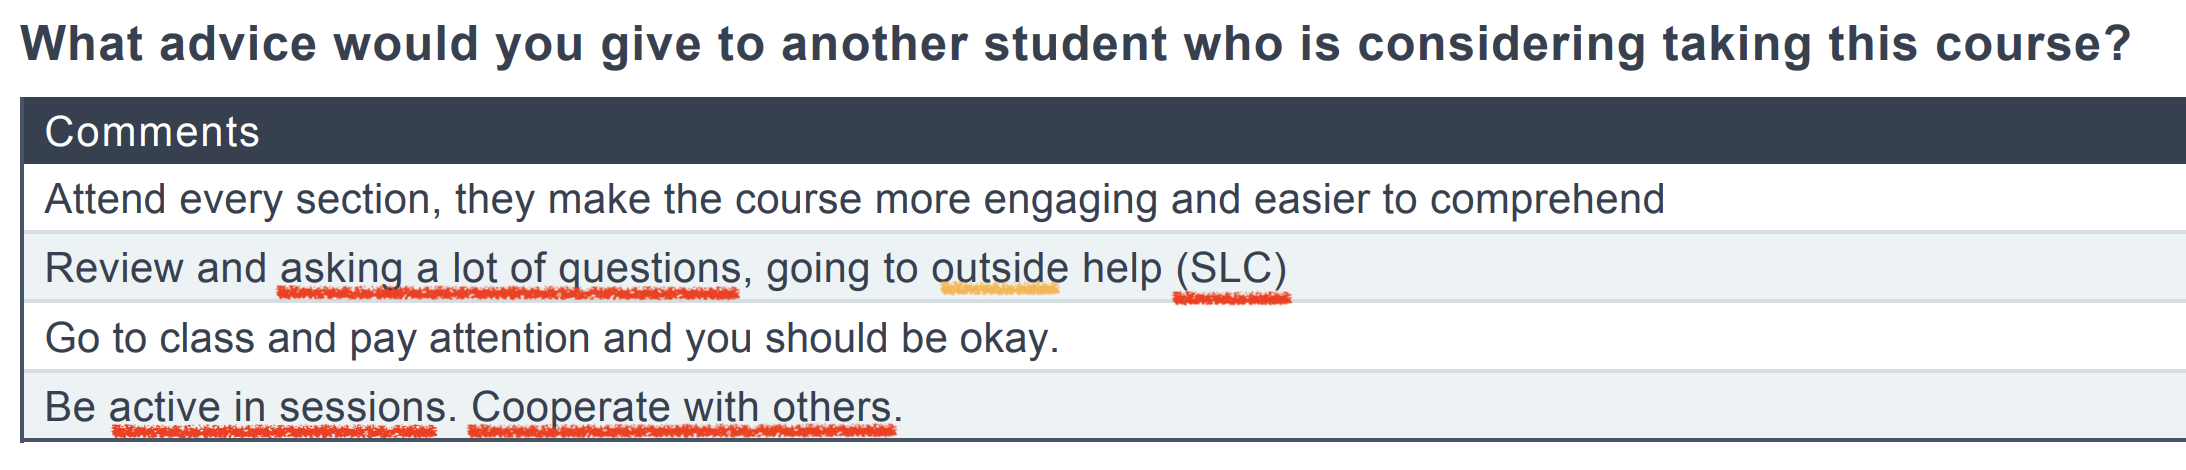
\includegraphics[width=\textwidth]{figures/Feedback/advice1.png}
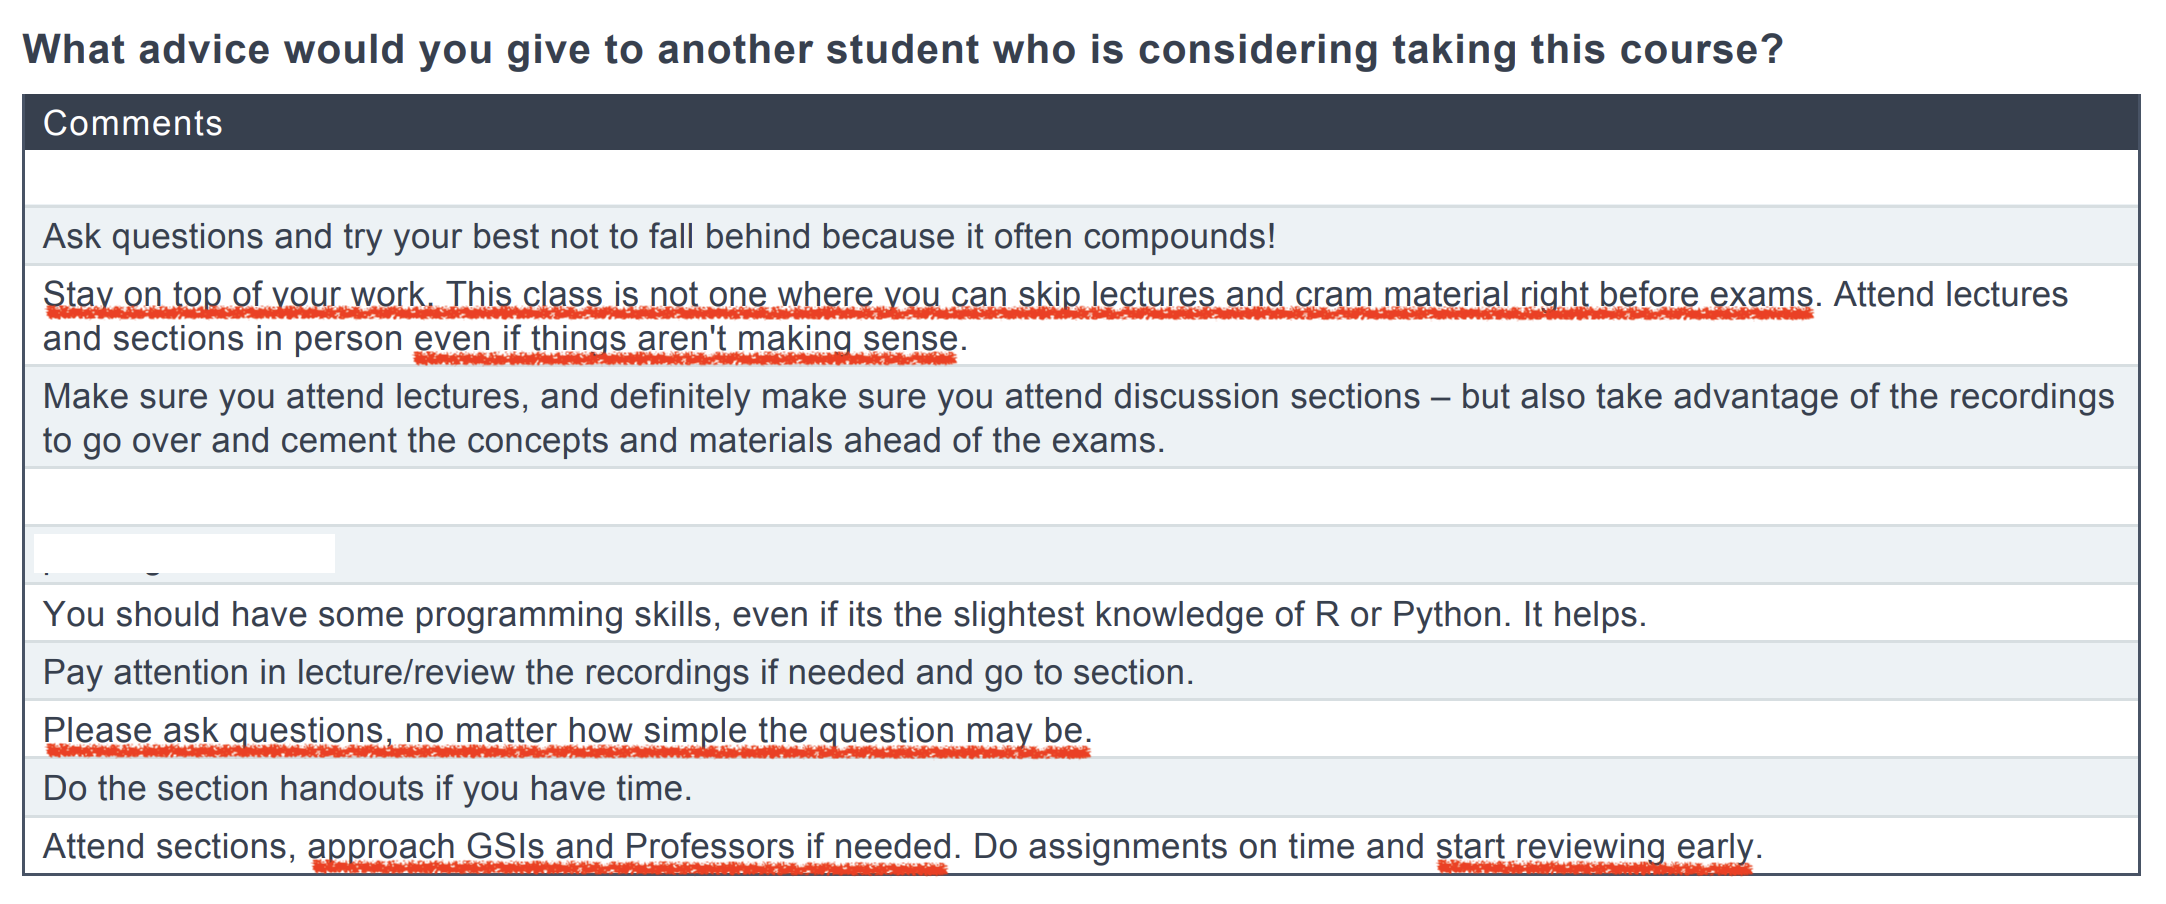
\includegraphics[width=\textwidth]{figures/Feedback/advice2.png}

\end{frame}


\begin{frame}{What your peers advise (2)!}

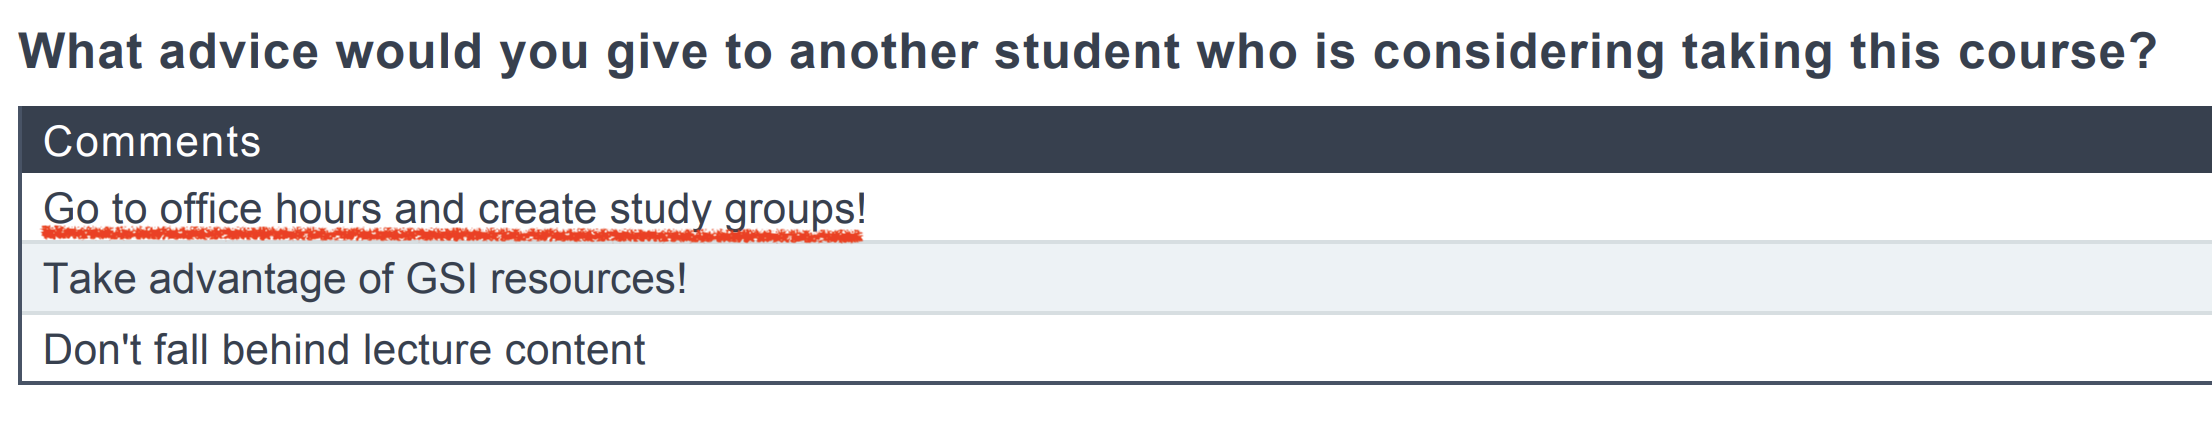
\includegraphics[width=\textwidth]{figures/Feedback/advice3.png}

\includegraphics[width=\textwidth]{figures/Feedback/advice4.png}

\end{frame}


\begin{frame}{What your peers advise (3)!}

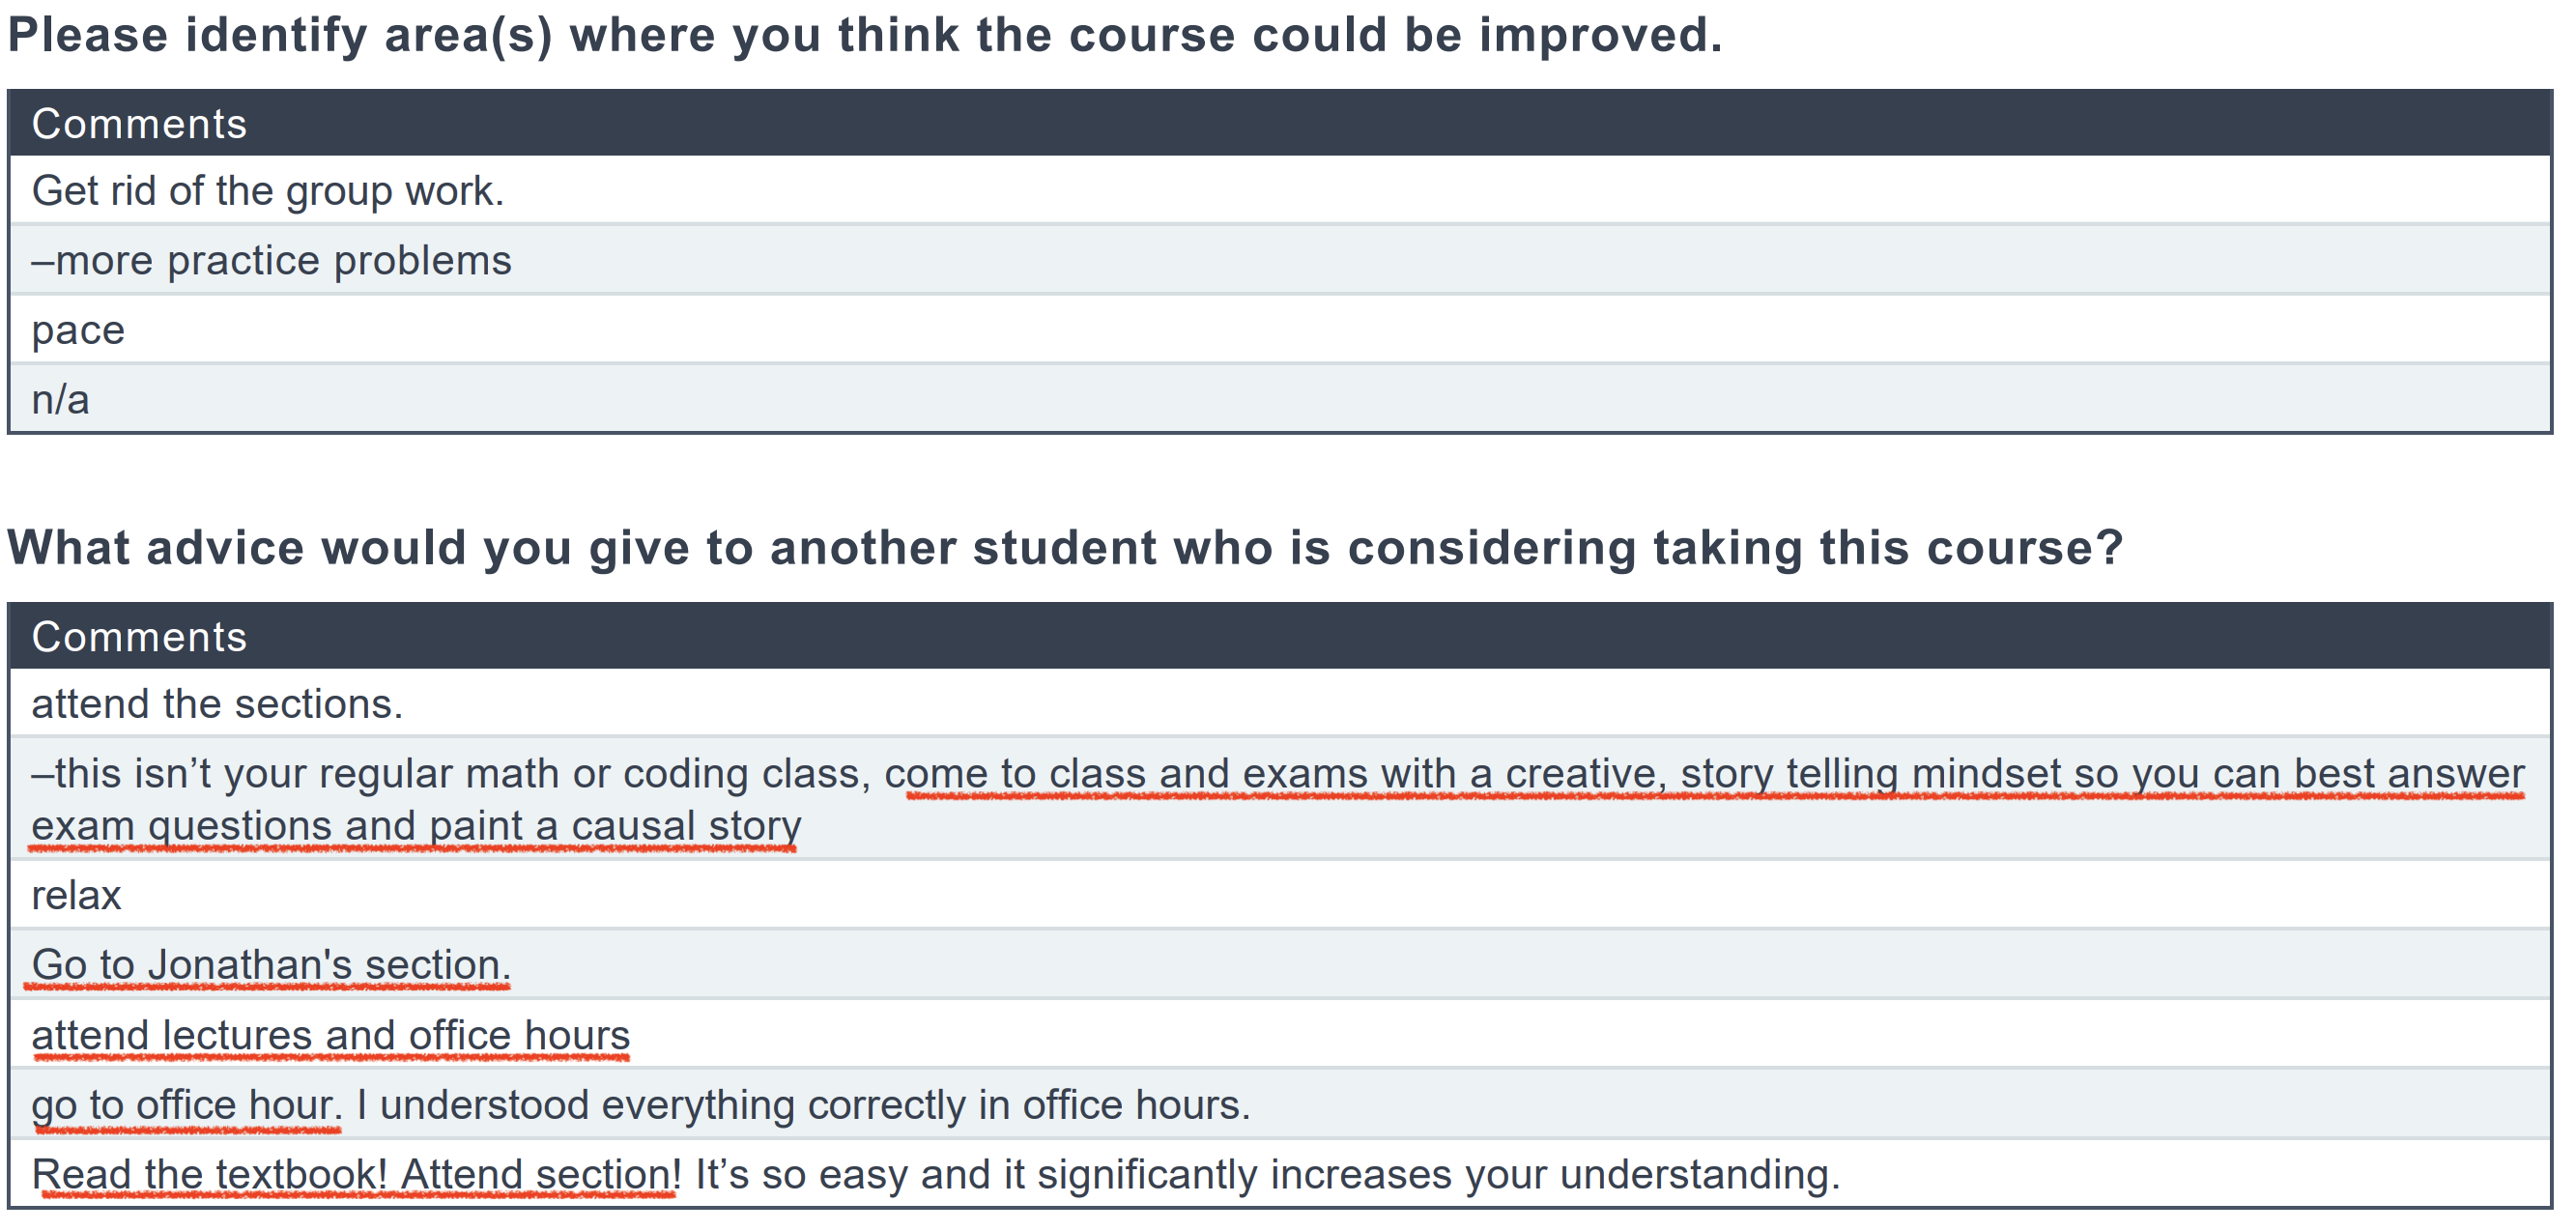
\includegraphics[width=\textwidth]{figures/Feedback/feedback_f2023_3.png}

\end{frame}





\begin{frame}{What your peers critiqued!}

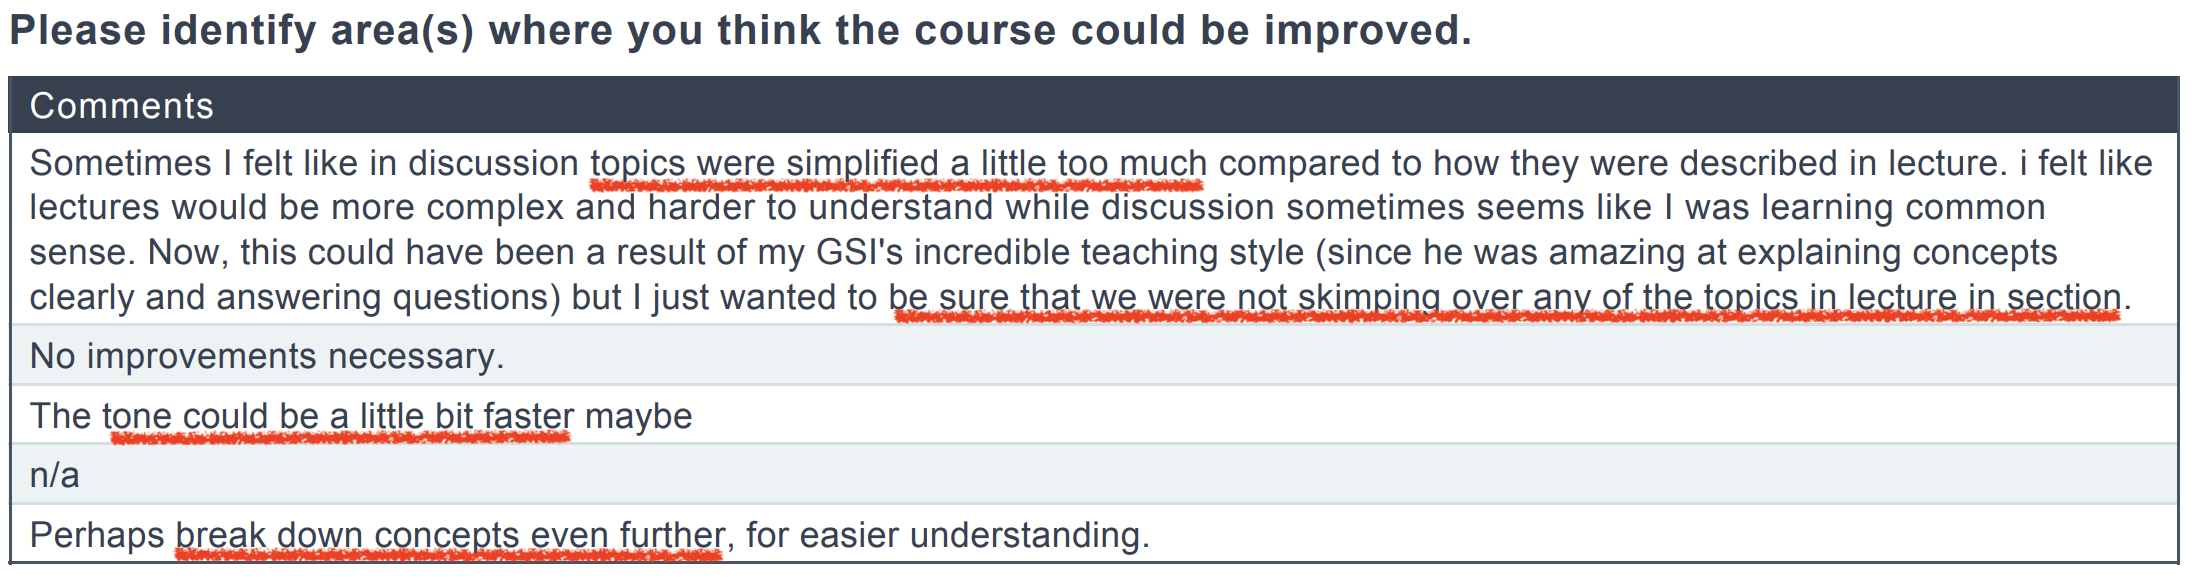
\includegraphics[width=\textwidth]{figures/Feedback/critique1.png}
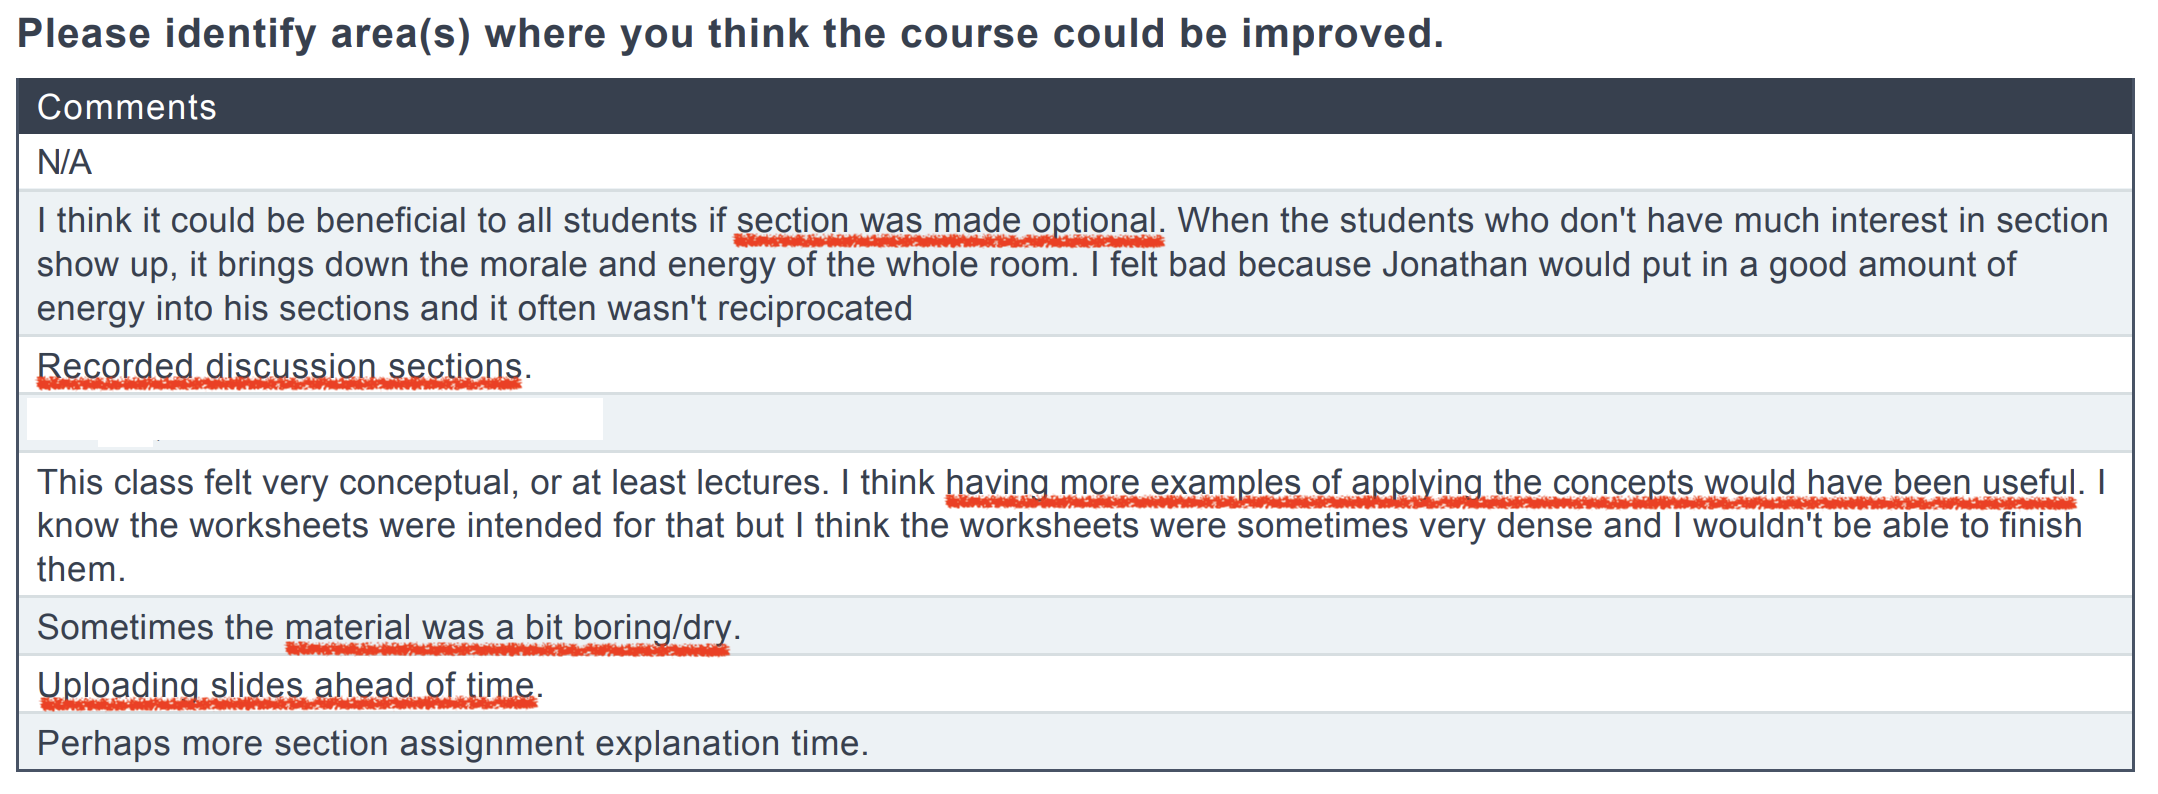
\includegraphics[width=\textwidth]{figures/Feedback/critique2.png}
\end{frame}


\begin{frame}{What your peers critiqued (2)!}
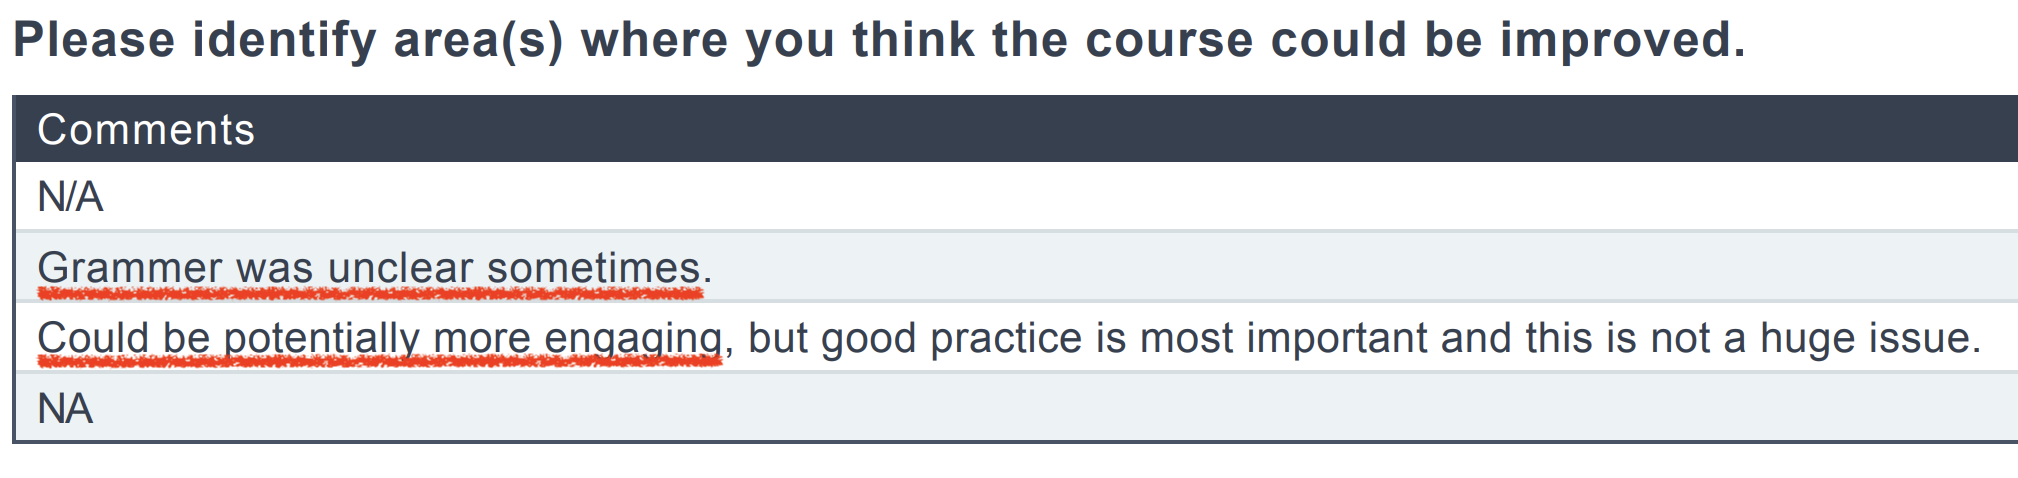
\includegraphics[width=\textwidth]{figures/Feedback/critique3.png}
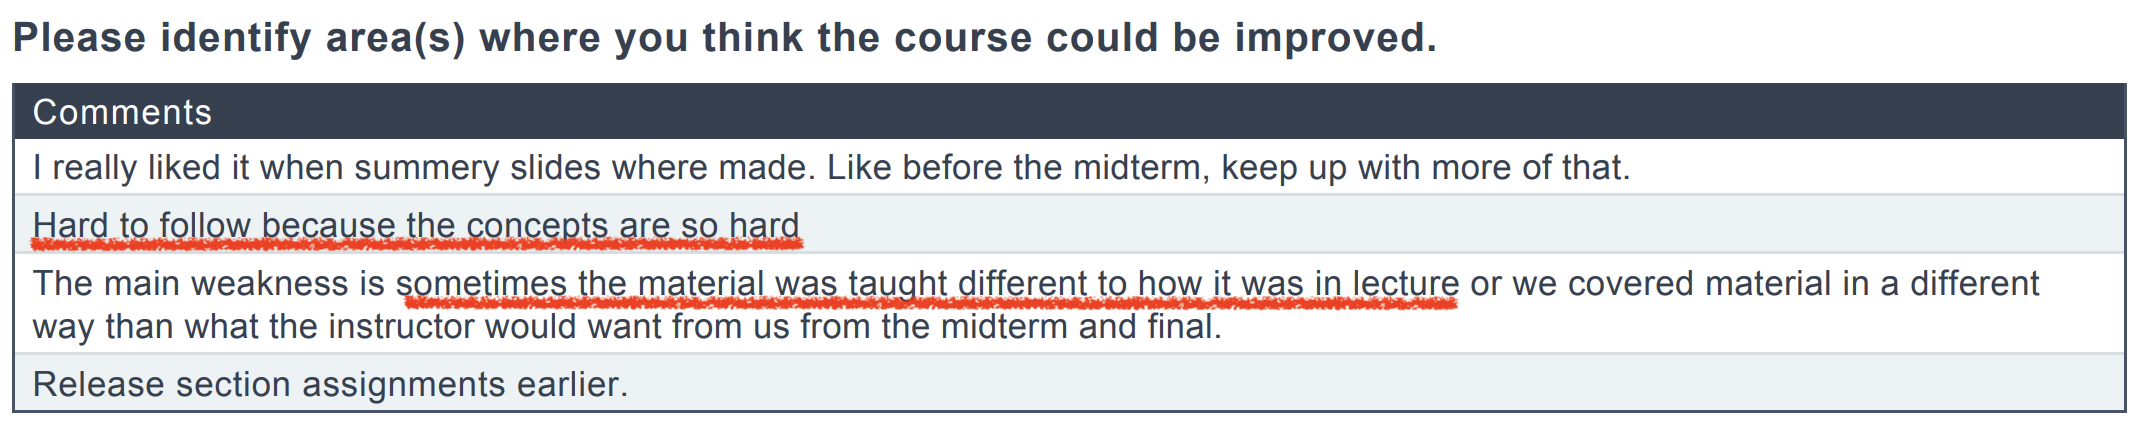
\includegraphics[width=\textwidth]{figures/Feedback/critique4.png}
\end{frame}


\begin{frame}{What your peers critiqued (3)!}
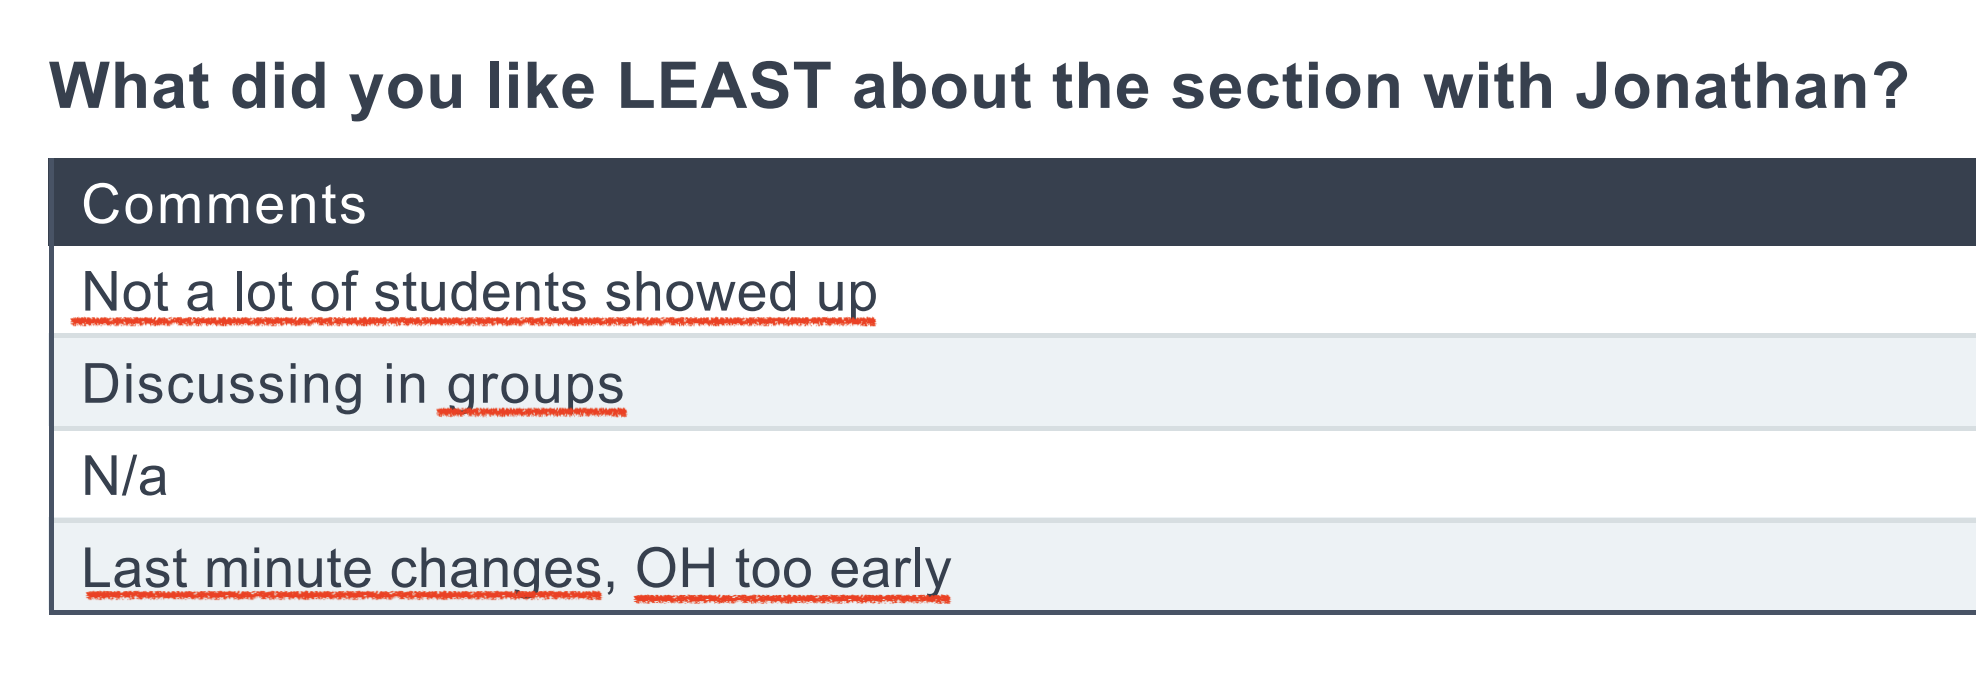
\includegraphics[width=\textwidth]{figures/Feedback/feedback_f2023_1.png}
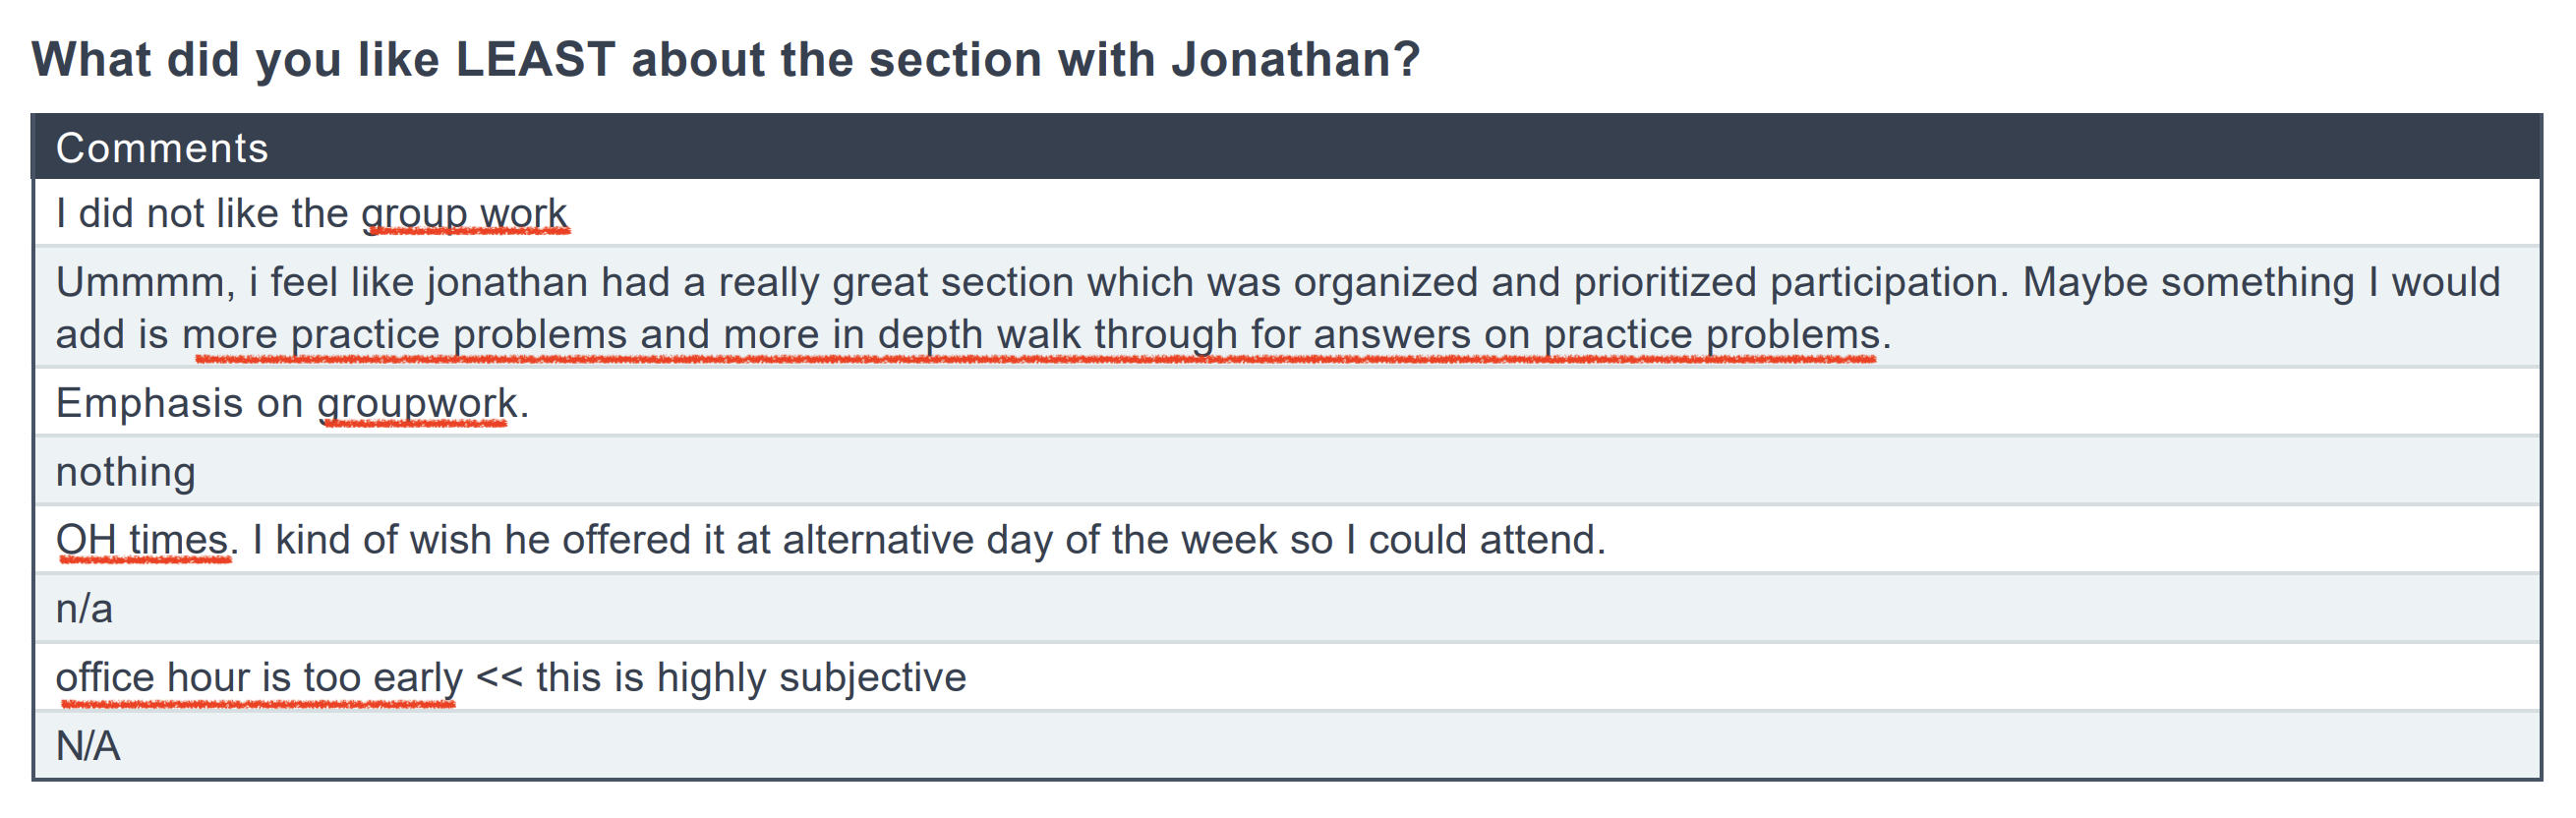
\includegraphics[width=\textwidth]{figures/Feedback/feedback_f2023_2.png}
\end{frame}




\begin{frame}{Newer feedback!}
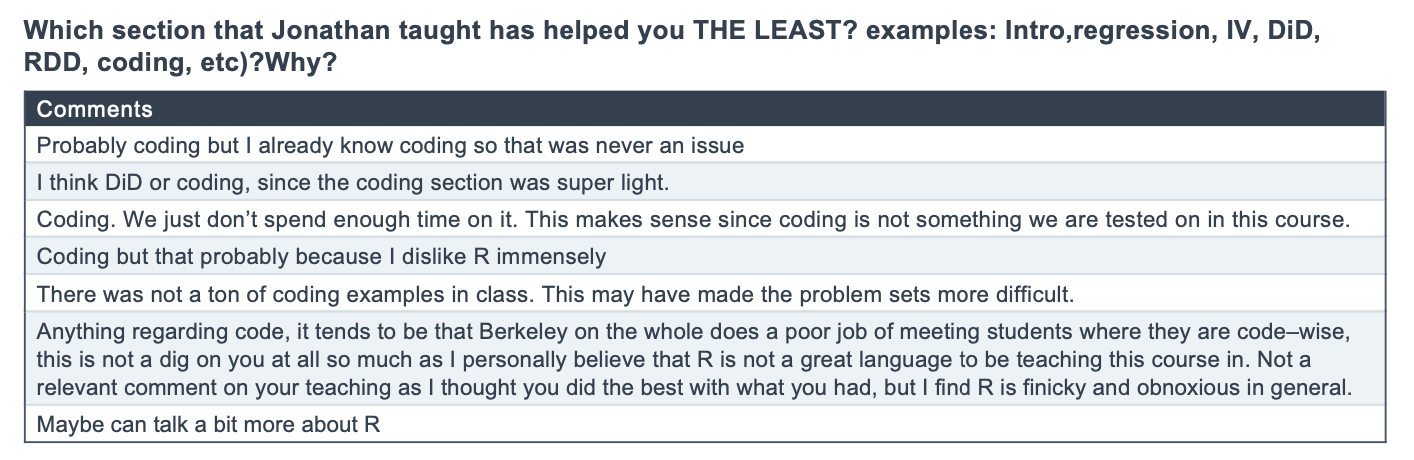
\includegraphics[width=\textwidth]{figures/Feedback/advice2024a.png}
\end{frame}


\begin{frame}{Newer feedback!}
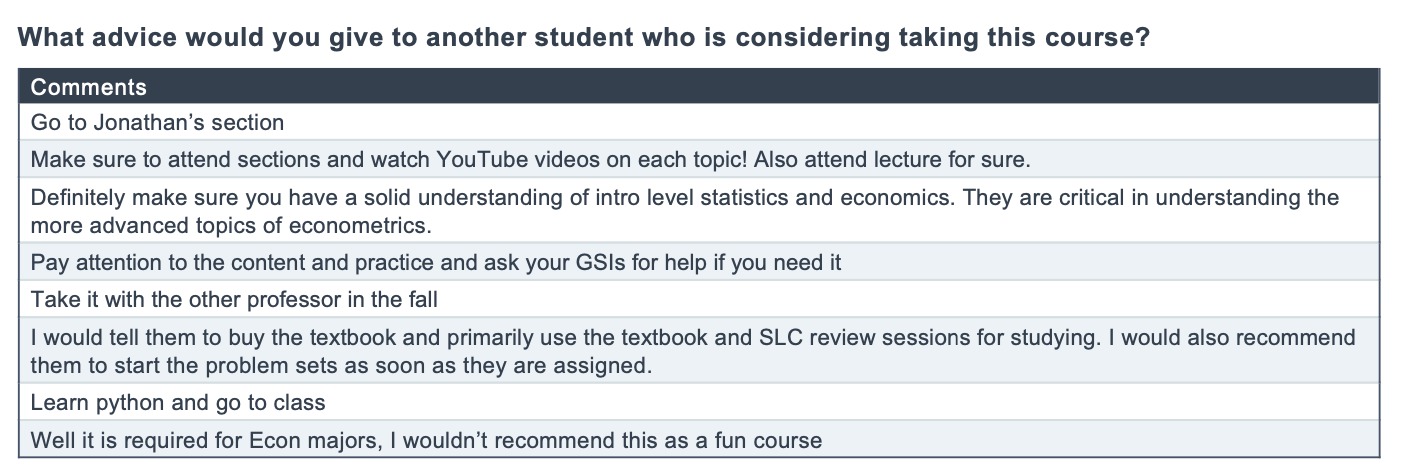
\includegraphics[width=\textwidth]{figures/Feedback/advice2024b.png}
\end{frame}



\begin{frame}{Newer feedback!}
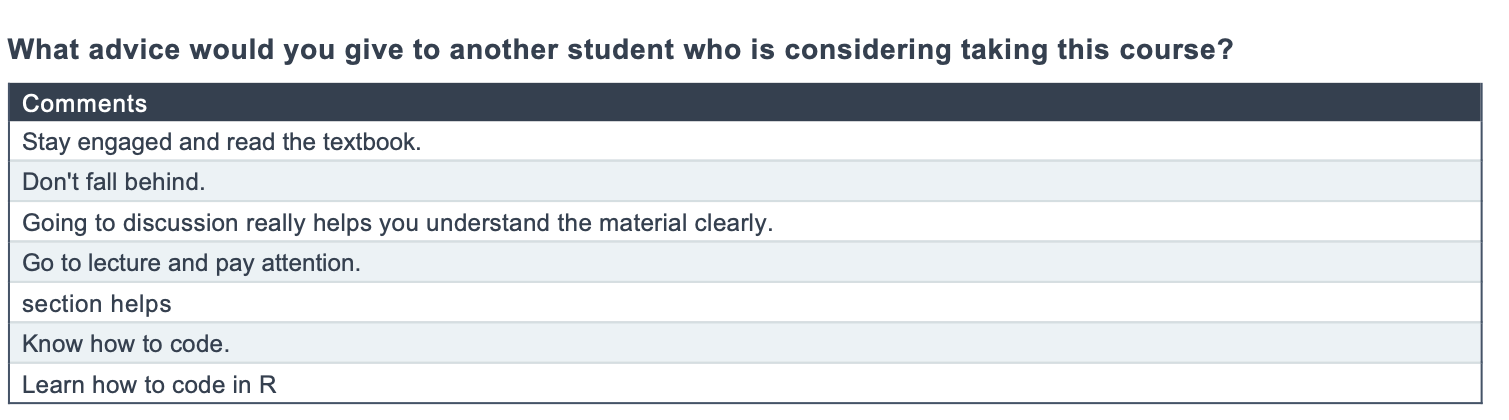
\includegraphics[width=\textwidth]{figures/Feedback/advice2024c.png}
\end{frame}




\questionslide




\section{Econ 140: The Big Picture}



\begin{frame}{The Big Picture}
Econometrics can help us
\begin{itemize}
    \item Understand causal relationships
    \item Critically consume news, research, claims
    \item Make decisions
\end{itemize}
in
\begin{itemize}
    \item Our private lives
    \item (Economic) Research
    \item Business
    \item Public Policy
\end{itemize}

\end{frame}





\begin{frame}{The Big Picture}
\begin{itemize}
\item Econometrics gives us amazing tools to answer economic questions, but also to answer any quantitative question based on data.
For example:
\begin{enumerate}
\item Will my outcomes be better if I invest my time into finding summer internships or into my coursework?
\item What is the effect of democracy on economic growth?
\item Will a firm make more money if it introduces pay-for-performance contracts?
\item Do minimum wages increase unemployment?
\end{enumerate}
In short: What is the effect of X on Y? \\
    %\item Why do we NOT use Excel? \href{https://www.theatlantic.com/business/archive/2013/04/forget-excel-this-was-reinhart-and-rogoffs-biggest-mistake/275088/}{A cautionary tale}
    \item Difference between econometrics and data science.
        \begin{itemize}
        \item Causality vs prediction (see \href{https://www.frontiersin.org/journals/bioengineering-and-biotechnology/articles/10.3389/fbioe.2016.00056/full}{here})
        \item Economic models
        \end{itemize}
\end{itemize}
\end{frame}





\section{Correlation and Causation}

\begin{frame}[fragile]{Dissecting Bad Causal Claims}

   \begin{alertblock} {\centering \vspace{-1.5ex} \\ Discuss in groups of 4: Why is this statement problematic?  \\ \vspace{-1.5ex} } \end{alertblock}

\begin{figure}
    \centering
    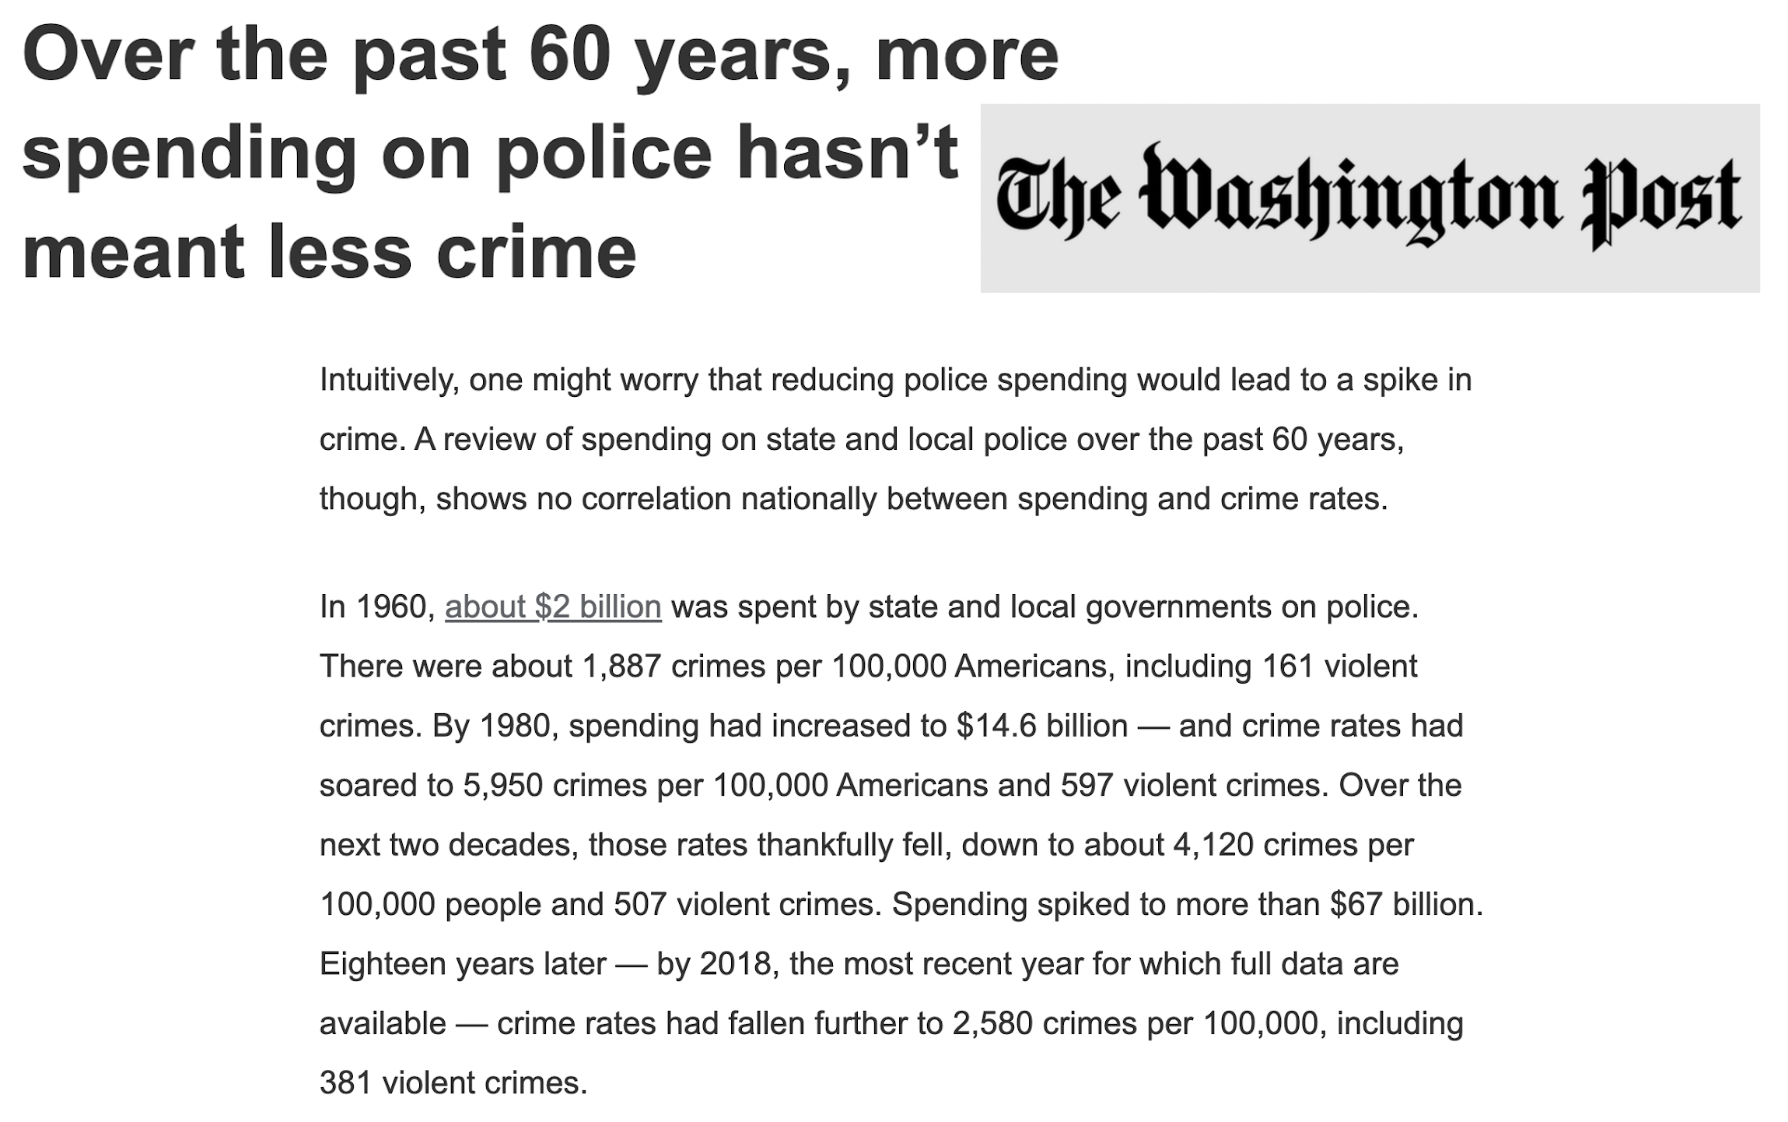
\includegraphics[width=0.75\textwidth]{figures/s1_washingtonpost.png}
    \caption{Police spending and Crime (\href{https://www.washingtonpost.com/politics/2020/06/07/over-past-60-years-more-spending-police-hasnt-necessarily-meant-less-crime/
}{Source})}
    \label{fig:wp}
\end{figure}


\end{frame}



\begin{frame}{Dissecting Bad Causal Claims II}

   \begin{alertblock} {\centering \vspace{-1.5ex} \\ Discuss in groups of 4: Why is this statement problematic?  \\ \vspace{-1.5ex} } \end{alertblock}

\begin{figure}[h!t]
    \centering    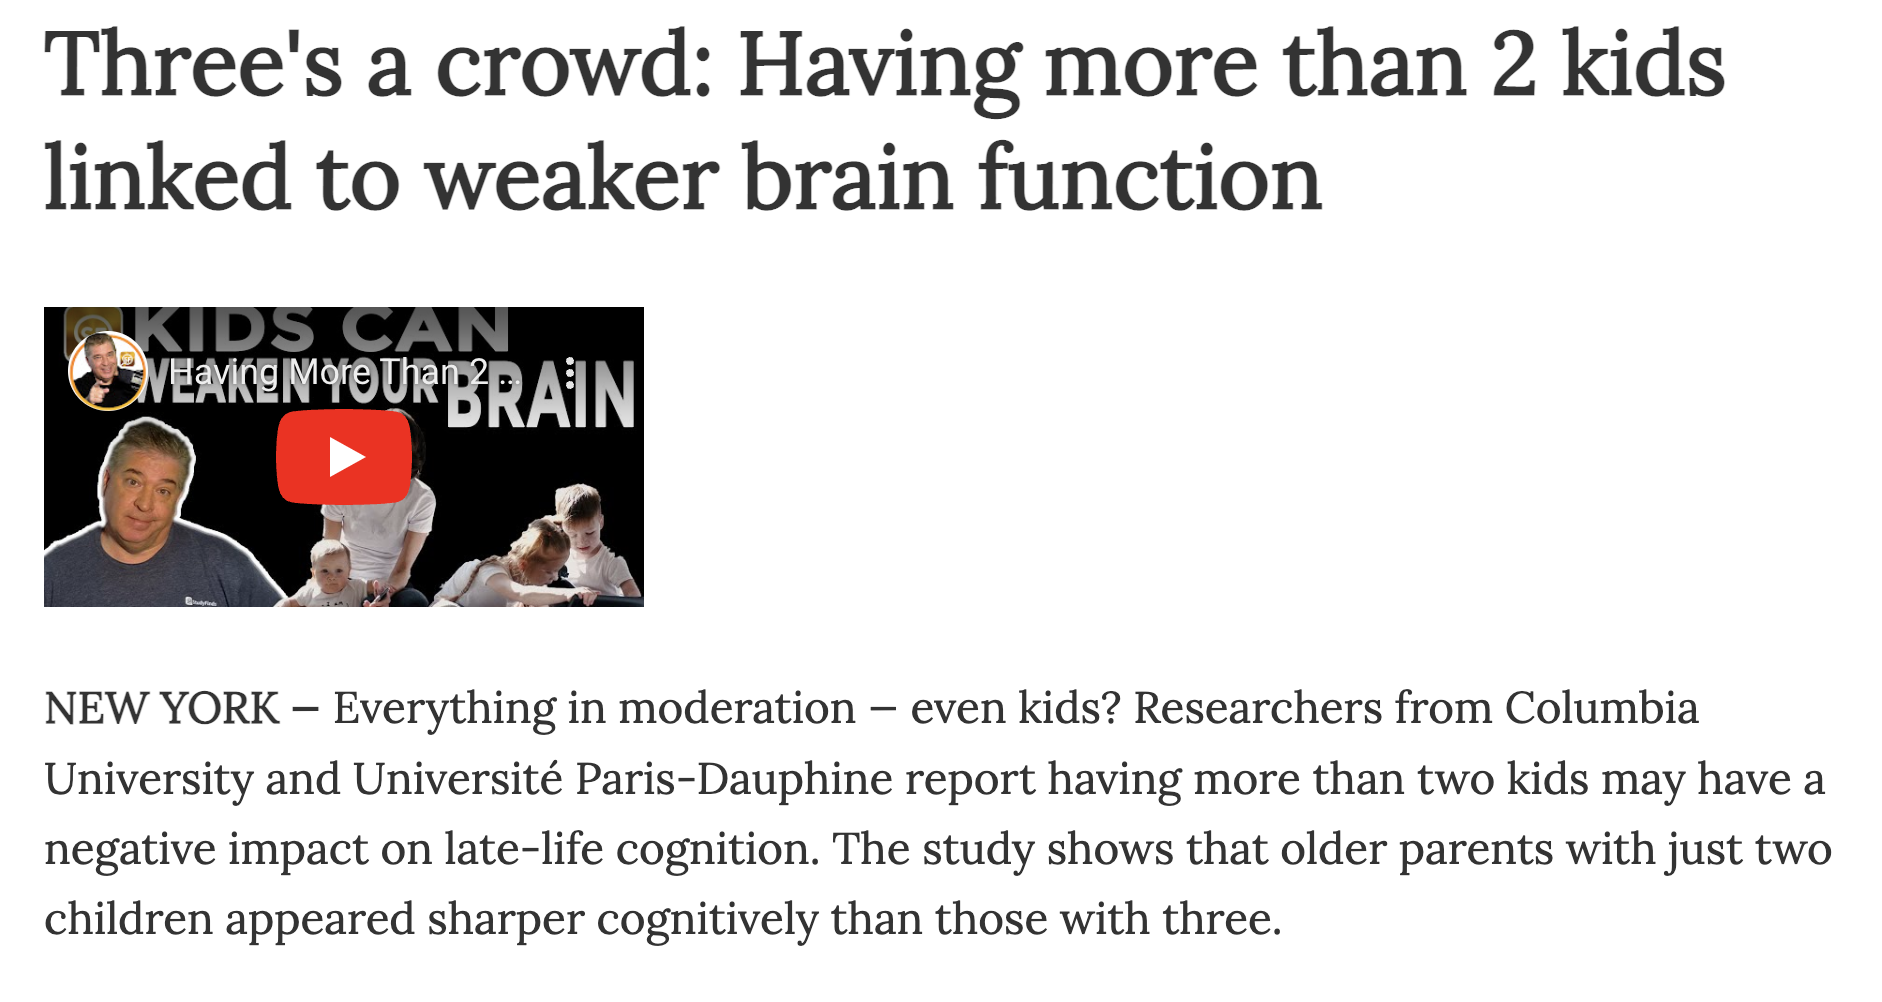
\includegraphics[width=0.8\textwidth]{figures/s1_brains.png}
    \caption{Number of Children and Cognitive Function(\href{https://studyfinds.org/too-many-kids-harmful-brain/
}{Source})}
    \label{fig:brain}
\end{figure}

\end{frame}






\begin{frame}{Dissecting Bad Causal Claims III}

   \begin{alertblock} {\centering \vspace{-1.5ex} \\ Discuss in groups of 4: Why is this statement problematic?  \\ \vspace{-1.5ex} } \end{alertblock}

\begin{figure}[h!t]
    \centering    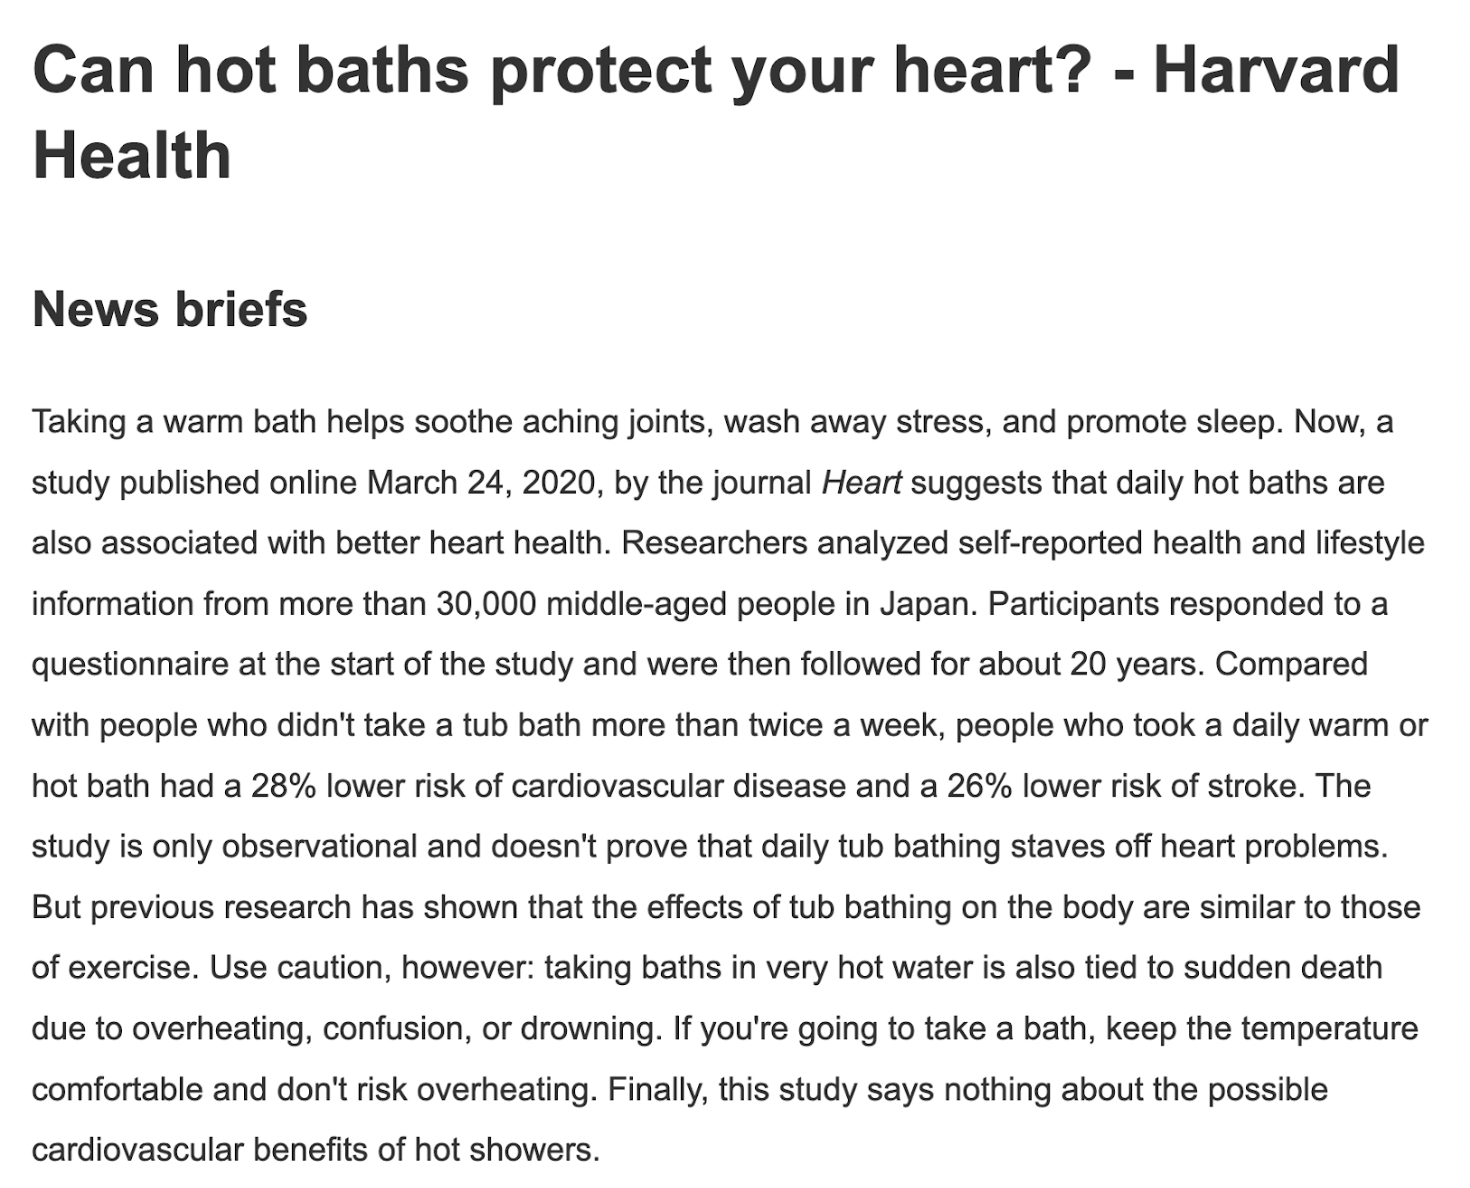
\includegraphics[width=0.65\textwidth]{figures/s1_harvard.png}
    \caption{Hot baths and health (\href{https://www.health.harvard.edu/heart-health/can-hot-baths-protect-your-heart}{Source})}
    \label{fig:bath}
\end{figure}

\end{frame}






\begin{frame}{Dissecting Bad Causal Claims IV}

\begin{alertblock} {\centering \vspace{-1.5ex} \\ Discuss in groups of 4: Why is this statement problematic?  \\ \vspace{-1.5ex} } \end{alertblock}

\begin{figure}[h!t]
    \centering    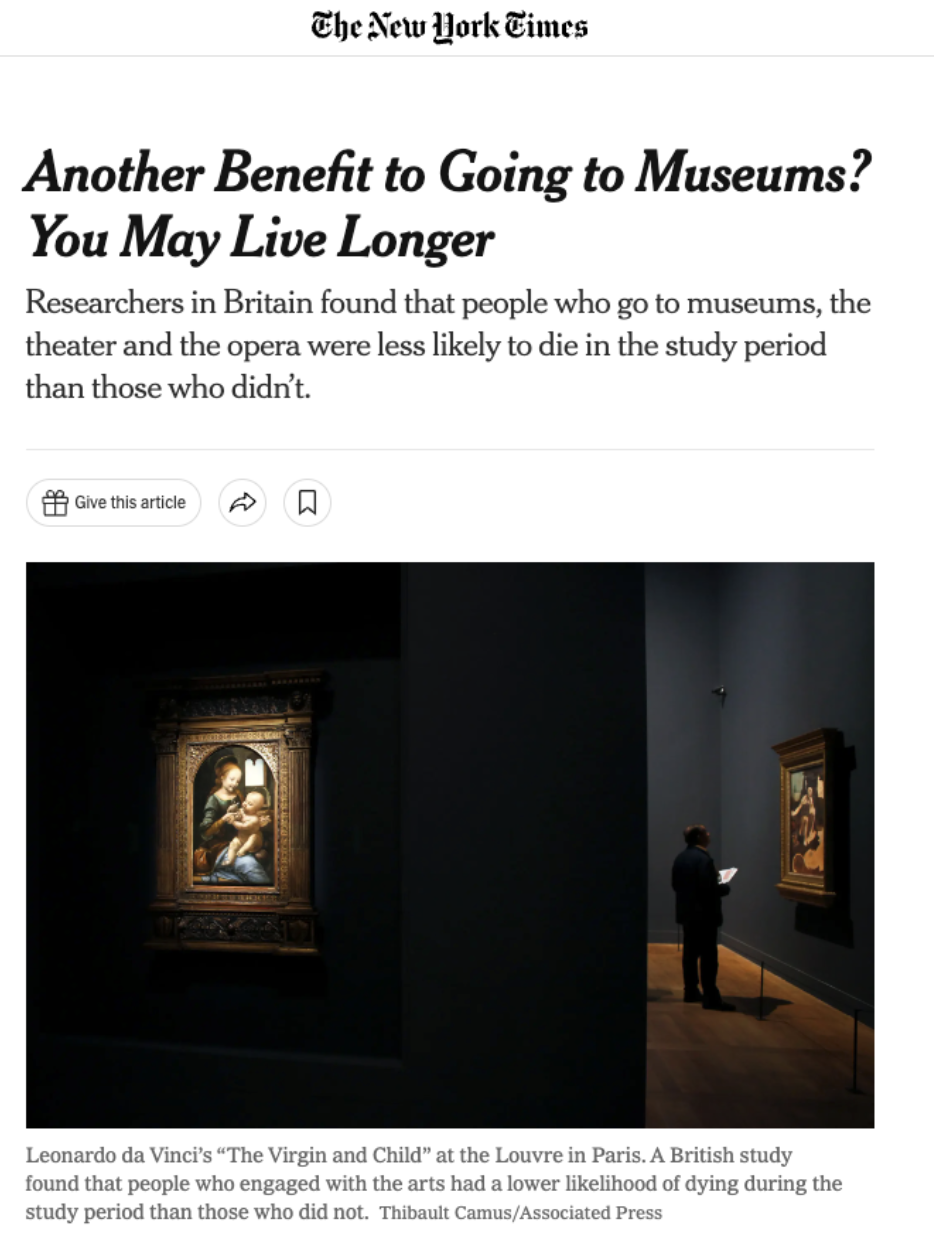
\includegraphics[width=0.42\textwidth]{figures/s1_nytimes.png}
    \caption{Museums and longevity (\href{https://www.nytimes.com/2019/12/22/us/arts-health-effects-ucl-study.html}{Source})}
    \label{fig:museum}
\end{figure}

\end{frame}








\begin{frame}{Dissecting Bad Causal Claims IV}

\begin{figure}[h!t]
    \centering    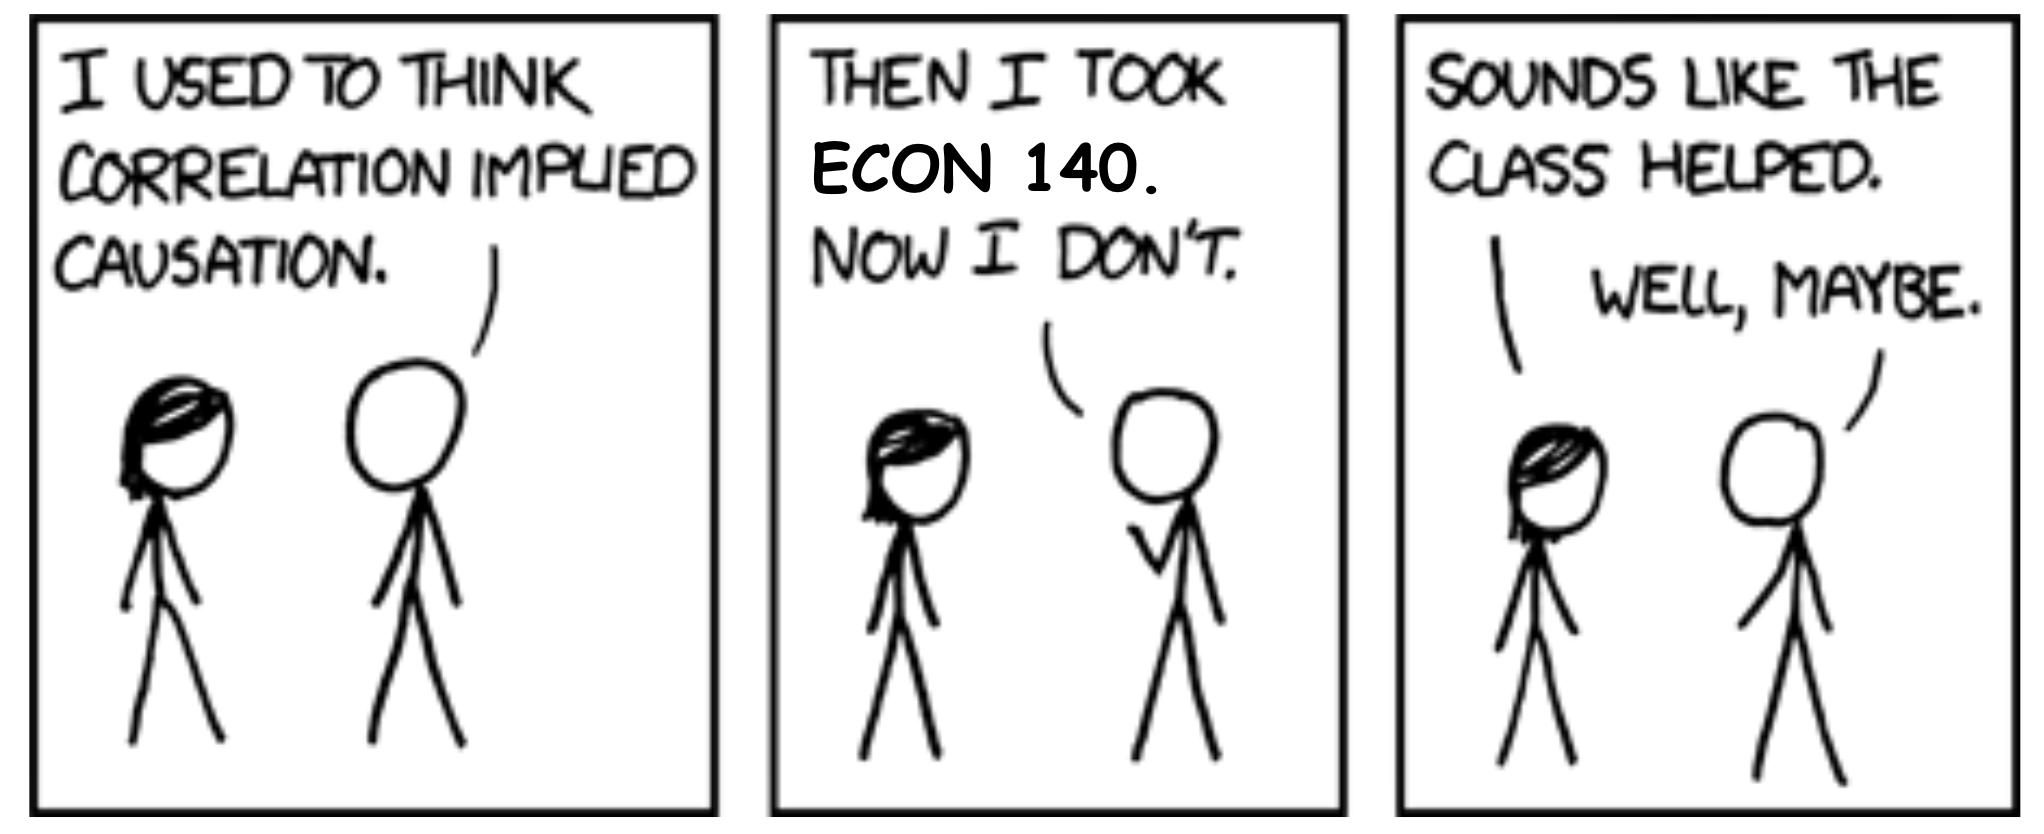
\includegraphics[width=1.0\textwidth]{figures/s1_meme.png}
    \caption{Correlation and causation}
    \label{fig:meme}
\end{figure}

\end{frame}

  




{\setbeamercolor{palette primary}{fg=black, bg=yellow}
\begin{frame}[standout]
    \raggedright
  Quiz Time! \\ \vspace{1cm}
  We have seen that \\
“Correlation Does  Not Imply Causation” \\
What about: \\
“No Correlation Implies No Causation”? \\

% \note{(Hint: Think about a car going up and down the hill, holding    its speed constant)}

\note{(Hint: Think about a car going up and down the hill, holding  its speed constant)}

\end{frame}
}




\end{document}
